\documentclass{beamer}
\usepackage[utf8]{inputenc}
\usepackage[french,noconfigs]{babel}
\usepackage{tikz}
\usepackage{ifthen}

\definecolor{Blue}{RGB}{0,59,92}
\definecolor{Grey}{RGB}{74,73,72}
\definecolor{Red}{RGB}{247,38,22}
\definecolor{DarkRed}{RGB}{197,26,27}
\definecolor{Yellow}{RGB}{223,176,0}
\definecolor{White}{RGB}{255,255,255}

\setbeamercolor{title}{fg=Blue}
\setbeamercolor{frametitle}{fg=Blue}
\setbeamercolor{structure}{fg=Blue}
\setbeamercolor{itemize/enumerate body}{fg=Grey}
\setbeamercolor{itemize/enumerate subbody}{fg=black}
\setbeamercolor{itemize subitem}{fg=Grey}
\setbeamercolor{normal text}{fg=DarkRed}
\setbeamercolor{section in toc}{fg=Grey}
\setbeamercolor{institute}{fg=Blue}
\setbeamercolor{footlinecolor}{fg=White,bg=Blue}



\setbeamertemplate{navigation symbols}{}
\setbeamertemplate{itemize items}[circle]

\title{Un test de présentation}
\author{Clément Durand}
\institute{École polytechnique}
\date\today

\newboolean{tocframe}\setboolean{tocframe}{false}

\makeatletter
\setbeamertemplate{footline}
{
	\leavevmode%
	\hbox{%
		\begin{beamercolorbox}[wd=.5\paperwidth,ht=2.25ex,dp=1ex,center]{footlinecolor}
			\usebeamerfont{title in head/foot}\insertsection
		\end{beamercolorbox}%

		\begin{beamercolorbox}[wd=.5\paperwidth,ht=2.25ex,dp=1ex]{footlinecolor}%
			\usebeamerfont{title in head/foot}\inserttitle \hfill \insertframenumber \,\,\,\,%
		\end{beamercolorbox}}%
		\vskip0pt
}
\makeatother

\AtBeginSection[]{
	{
        \makeatletter
        \setboolean{tocframe}{true}
		%\setbeamertemplate{background canvas}{}%
        %\setbeamertemplate{background canvas}{\tikz[remember picture,overlay]\node[opacity=0.2] at (current page.east) {\includegraphics[width=8cm,keepaspectratio]{./img/blazon}};}
		\setbeamertemplate{footline}{}
        \makeatother
		\begin{frame}
			\frametitle{Table of Contents}
			\tableofcontents[currentsection]
			\addtocounter{framenumber}{-1}
		\end{frame}
        \setboolean{tocframe}{false}
	}
}


\begin{document}

{
\setbeamertemplate{background canvas}{\tikz[remember picture,overlay]\node[shift={(-1.25cm,1.25cm)},opacity=0.8] at (current page.south east) {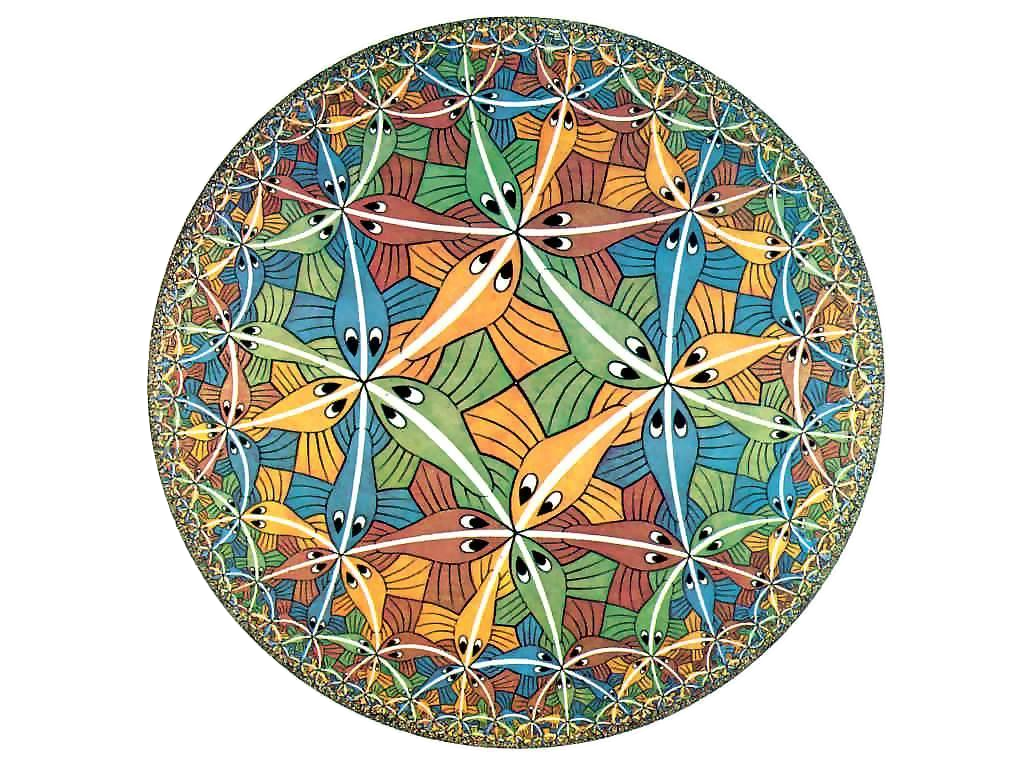
\includegraphics[width=8cm,keepaspectratio]{./img/escher1}};}

\frame[plain]{\titlepage}
}

\begin{frame}
Hello World~:
\end{frame}

\setbeamertemplate{background canvas}{%
\ifthenelse{\boolean{tocframe}}{%
\tikz[remember picture,overlay]\node[opacity=0.2,left=-4pt] at (current page.east) {\includegraphics[height=0.9\paperheight,keepaspectratio]{./img/halfblazon}};%
}{%
\tikz[remember picture,overlay]\node[shift={(-1cm,-1.25cm)},opacity=0.5] at (current page.north east) {\includegraphics[width=1.25cm,keepaspectratio]{./img/blazon}};%
}}

\section{Introduction}

\begin{frame}
Hello World~:
\end{frame}

\section{Background}
	\subsection{frame 1}
		\begin{frame}{frame 1}
			\begin{itemize}
			\item Item A
			\item Item B
			\begin{itemize}
			\item Subitem 1
			\item Subtem 2
			\end{itemize}
			\item Item C
			\end{itemize}
		\end{frame}


\end{document}